\chapter{Anwendung}\label{ch:anwendung}

Um mithilfe der Playbooks aus diesem Projekt einen Kubernetes-Cluster einzurichten, müssen Material und Infrastruktur vorbereitet werden.
Anschließend werden die SD-Karten einzeln mit Raspbian beschrieben und mit dem Playbook \texttt{local-""raspbian.yaml} für den Headless-Betrieb konfiguriert.
Sobald alle Raspberry Pis online sind, wird Kubernetes mit dem Playbook \texttt{kubernetes.yaml} aufgesetzt.

% https://www.draw.io/?title=ansible-kubernetes-anwendung#R7Vlbm5owEP01PNpPiIo%2BVte91K11a%2FfWtygRsgZiQ%2FCyv75BgoDZVbxrv774kWESnDNzToaggYY7vWFw5HynFiKaUbSmGrjSDKNimuI3NMwiA6gUI4PNsBWZ9MTQxe9IGmO3AFvIzzhySgnHo6yxTz0P9XnGBhmjk6zbgJLsU0fQRoqh24dEtT5jizuRtWqYif0WYduJn6xXatEdF8bOMhLfgRadpEygqYEGo5RHV%2B60gUiIXYzL893smdwPKzffHvw%2F8LHe%2BtV%2BKkSLXW8yZRECQx7feukfrz58%2FPowfLdNd6xXS7Wnh5eCjHUMSSDxkrHyWQwgsgSeckgZd6hNPUiaibXOaOBZKHxMUYwSn3tKR8KoC%2BMb4nwmiwMGnAqTw10i7%2BaMT%2BLg04D10YqggCwzyGzEV%2FhVI78wwFStSPRuEHURZzPhwBCBHI%2BzBQVlXdoLvwR7cSHh3yAVQEnFT%2BiPehh6YdkT6DvIU5KTQB%2FiOHEwR90RnKMzEXTeBeYxYhxNVwIT35UEkQqhAzmeJHzTYx8nxbXYb%2F9QglNUMZpi%2FhJO%2F1KWo9fUnaupXHk%2BmMUDT8SbmhQOX9P3kmnzUTxvz4yp5mQMMM6KMlWFMh0CZz1Kh5pRISKQeo%2BJK5vPEYssAyoQE4SCEpDKnyAU8HpDYISRcC%2B20SQxx9MJFVtKgS0YGS0m%2FnW0XvYZyVNh4A%2B0BtDqDYddCn2rOelbPhR99dp%2F%2Bm5EXz3vjgfOir6Lxuq4ed4yZ9vUx2Z5Xps%2B%2FeP8ZStk2Grf3tV%2BD4zrojtp12%2Freku2hjvkWU7tUDxXz1g5SlnpWN7Qo4DkpHRrurROpZxZprS0TBSdssy85hbB7CA3aufVvSq0oNDPcGrYft1jL5gWOo0Qe%2BwRZF%2BIlps5pXwZ8f11YuVTSrmeImpC282kXD%2BulMcd1nopL52Vlsf%2FewWJOjhDn5BMolXjF0KlRbtzsrYIVBSIPYRV9I7ZK21DMD1NrxTbjkSw0m6b7ckIpr7svMHLE9fLyD0wzyv3JVVcsWeFjyIEzaXVF782muupCOxalVSHur3AXy%2BnkGDbE9d9Abl4HT6gvppZgc2rr9WD6aupoHyw44Rh0EPMQxz5%2F9RRAjCyOY0b%2B2PsmZ%2B%2F92SJI8jPVd0kBI98lBc5BZG8YOY%2BhDli4%2F4hcLoCXFOU1%2Fnhtlxxi1fSkyFnnLQhO9rhlXIGsb9d2lR36c9rdO%2BHGmb2MEI38p1GKOuA5YWWK%2B6T05H1xxpimHx1jNyTT7eg%2BRc%3D
% TODO start und ende?
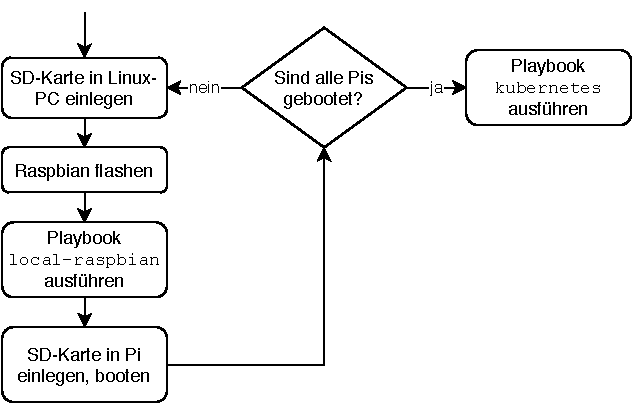
\includegraphics[width=.7\textwidth]{img/anwendung.pdf}

\section{Vorbereitung}\label{sec:vorbereitung}
Zum erfolgreichen Ausführen dieser Anleitung müssen folgende Voraussetzungen erfüllt sein:

% TODO lieber absätze
\begin{itemize}
    \item \textbf{Raspberry Pis} in beliebiger Anzahl und ebenso viele Speicherkarten und Netzteile stehen bereit.
    \item \textbf{Ein Linux-Rechner} steht bereit, um die Speicherkarten zu flashen und die Ansible-Playbooks auszuführen. Dafür sind Balena Etcher\footnote{\url{https://www.balena.io/etcher/} -- \today} und Ansible\footnote{\url{https://www.ansible.com/} -- \today} installiert, das Git-Repo zu diesem Projekt mit den Verzeichnissen \texttt{inventory} und \texttt{playbook} ist ausgecheckt und ein Image von Raspbian Lite\footnote{\url{https://downloads.raspberrypi.org} -- \today} ist heruntergeladen.
    % https://downloads.raspberrypi.org/raspbian_lite/images/raspbian_lite-2020-02-14/2020-02-13-raspbian-buster-lite.zip
    \item \textbf{Ein Terminal} mit \texttt{playbook} als Current Working Directory ist geöffnet.
    \item \textbf{Ein WiFi-Access Point} mit Internetzugriff ist in Betrieb. Seine Einstellungen (IP, SSID, WPA2-Key) entsprechen den Angaben in den Dateien \texttt{inventory/""group\_vars/""all.yaml} und \texttt{playbook/""local-""raspbian.yaml}. Der zuvor erwähnte Rechner ist mit dem Access Point verbunden.
    \item \textbf{Die Inventory-Datei} \texttt{inventory/""k8s-cluster.yaml} bildet den derzeitigen Cluster ab -- enthält also keine Einträge unter \texttt{hosts}, falls ein neuer Cluster eingerichtet werden soll:

        \begin{lstlisting}
nodes:
  hosts:
        \end{lstlisting}
        \caption{Leere Inventory-Datei}
\end{itemize}

Die benötigte Zeit für die gesamte Einrichtung beträgt ca. 10 Minuten pro Raspberry Pi plus ca. 30 Minuten für den gesamten Cluster.

\section{Raspbian installieren}\label{sec:raspbian-installieren}
Die Schritte in diesem Abschnitt müssen für jeden Raspberry Pi einzeln durchgeführt werden.

\begin{enumerate}
    \item Speicherkarte in den Linux-Rechner einlegen.
    \item Raspbian-Image mit Balena Etcher auf die Speicherkarte flashen.
    \item Raspbian-Playbook ausführen:
        \begin{lstlisting}
ansible-playbook -i ../inventory/k8s-cluster.yaml local-raspbian.yaml
        \end{lstlisting}
        \caption{CLI-Befehl zur Ausführung des Raspbian-Playbooks}
    \item Speicherkarte in den Raspberry Pi einsetzen und booten.
\end{enumerate}

\section{Cluster aufsetzen}\label{sec:cluster-aufsetzen}

Wenn alle Raspberry Pis gestartet sind, wird die Installation mit dem Kubernetes-Playbook fortgesetzt:
\begin{lstlisting}
ansible-playbook -i ../inventory/k8s-cluster.yaml kubernetes.yaml
\end{lstlisting}
\caption{CLI-Befehl zur Ausführung des Raspbian-Playbooks}

Der Kubernetes-Cluster ist anschließend einsatzbereit.

\section{Weitere Nodes hinzufügen}\label{sec:weitere-nodes-hinzufügen}

Sollen zu einem fertigen Cluster weitere Nodes hinzugefügt werden, kann auch dafür diese Anleitung verwendet werden.
Die Inventory-Datei darf dann nicht leer sein, sondern muss die bereits vorhandenen Nodes enthalten.
